\section{Planare Rekonstruktion}

Wie bereits in Absatz \ref{sec:polygon_reconstruction} beschrieben, lässt sich das Problem der Optimierung von Augmented Reality mit Hilfe von Tiefeninformationen auf eine Echtzeit Rekonstruktion zurückführen. Im Gegensatz zur Rekonstruktion komplexer Oberflächen, mit dem vorgestellten TSDF Verfahren, soll hier eine Idee näher erläutert werden, die eine Rekonstruktion allein auf planaren Primitiven ermöglicht. \citet{yang2010plane} erwähnt hierzu, dass Ebenen in fast allen künstlichen Umgebungen zu finden sind und auf Grund ihrer vorteilhaften geometrischen Eingenschaften in verschiedensten Computer Vision Verfahren verwendet werden. Daher gibt es viele Forschungsarbeiten, Methoden und Algorithmen um aus verschiedensten Informationsquellen ein Ebenenmodell zu extrahieren.\\

Wie in dem \enquote{Simultaneous Localization and Mapping} (SLAM) Verfahren von \citet{trevor2012planar} wird hier zunächst eine Ebene in der Pointcloud mit Hilfe des RANSAC Algorithmus gesucht. RANSAC bietet gegenüber anderen Algorithmen zur Ebenen Detektion den Vorteil, ein Modell auch bei vielen Ausreißern performant zu ermitteln. Agglomeratives Clustering und Region Growing wie von \citet{feng2014fast} beschreiben, eignet sich auf Grund des Ausgabeformats aus Project Tango nicht, da es keine organisierte Point Cloud ausgibt. \\

Die Repräsentation der Ebene \(P\) wird, angelehnt an das Vorgehen von \citet{trevor2012planar}, wie in Gleichung \ref{eq:plane} festgehalten. Dabei handelt es sich um den Normalenvektor \(\vec{n}\) und der Distanz zum Ursprung \(d\) der Hesse Normalform einer Ebene, sowie der Punkte der konvexen Hülle \(H\). Um die konvexe Hülle der Ebene zu bestimmen, wird der Graham Scan Algorithmus verwendet. Wie auch von \citet{trevor2012planar} beschreiben wird die konvexe in der Repräsentation festgehalten, um eine sukzessive Verbesserung einer Ebene nach mehreren Messdurchläufen zu ermöglichen. So werden die Punkte der konvexen Hülle pro Messvorgang kombiniert, damit die Ebenenausbreitung auch außerhalb des Sichtfeldes beibehalten werden kann.

\begin{equation} \label{eq:plane}
P=\left[\vec{n}, d, H\right] \qquad H=\vec{h_1}, \vec{h_2}, \ldots  \vec{h_n}
\end{equation}

Um wiederum aus dieser Repräsentation eine Triangulation zu erhalten, wird hier die zweidimensionale Sweep-Line Delaunay Triangulation durchgeführt. Die Schritte aus dem Algorithmus \ref{lst:planeReconstruction} werden in den folgenden Kapiteln näher beschreiben.

\begin{lstlisting}[mathescape,caption=Algorthmus der planaren Echtzeit Rekonstruktion, label=lst:planeReconstruction]

Eingabe: Octtree $O$
Ausgabe: Polygonpunkte $T_{Gesamt}$

für jedes Cluster $C$ aus $O$
    bestimme Ebene [$\vec{n}$, $d$, $P$] mit RANSAC aus $C_{Punkte}$
    wenn keine Ebene mit genügend $P$ in $C_{Punkte}$ gefunden wurde
    		nächstes Cluster (continue)
    wenn Ebene mit [$\vec{n}$, $d$, $H_{alt}$] in $C_{Ebenen}$ existiert	
        füge die konvexe Hülle $H_{alt}$ zu $P$ hinzu	
    bestimme die konvexe Hülle $H_{neu}$
    bestimme die Tringulation $T_{Ebene}$ aus $H_{neu}$
    $T_{Gesamt}$ += $T_{Ebene}$
    $C_{Ebenen}$ += [$\vec{n}$, $d$, $H_{neu}$]
    $C_{Punkte}$ - $P$
		

\end{lstlisting}

\subsection{RANSAC zur Ebenendetektion}

Der \enquote{RAndom SAmple Consensus} Algorithmus (RANSAC), vorgestellt von \citet{fischler1981random}, ist in der Lage, aus einer Menge von Daten mit vielen Ausreißern, die Parameter für ein passendes Modell zu schätzen. Anders als andere Schätzverfahren wie \enquote{Least-Median} oder \enquote{M-Schätzer}, welche aus der Statistik Literatur entnommen und entsprechend angepasst wurden, wurde RANSAC speziell für die Anwendung in der Computer Graphik entwickelt. Der Kern dieses Algorithmus ist das wiederholte Bestimmen eines Modells aus zufälligen und für das Modell ausreichenden Stichproben. Listing \ref{lst:ransac} zeigt den Verlauf des RANSAC Algorithmus. Die Anzahl der Iterationen \(N\) hängt dabei allein von dem Anteil der Ausreißer in den Messwerten ab. Daher sollte sie entsprechend gewählt werden, um die Wahrscheinlichkeit zu verringern, dass Ausreißer in den Stichproben enthalten sind. \citep{derpanis2010overview} \\

\begin{lstlisting}[mathescape,caption=Der RANSAC Algorithmus, label=lst:ransac]
Eingabe: Messwerte $P$, Modelltoleranz $e$, maximale Iterationen $N$
Ausgabe: Modell $m$, Unterstützende Messwerte $P_m$

1. Wähle zufällig so viele Stichproben aus den Messwerten $P$,
   wie nötig sind, um das Modell zu bestimmen
2. Bestimme aus den gewählten Stichproben das Modell $m$
3. Ermittle die Anzahl der Messwerte $P$, die mit einer 
   entsprechenden Toleranz $e$ das ermittelte Modell $m$ 
   unterstützen
4. Wenn prozentual genügend Messwerte aus $P$ das Modell $m$ 
   unterstützen, ermittle aus den unterstützenden Messwerten 
   $P_m$ durch lineare Regression erneut das finale Modell 
   $m$ und terminiere
5. Wiederhole die Schritte 1-4 $N$ mal
\end{lstlisting} 

Um mit dem RANSAC Algorithmus Ebenen in einer Punktewolke bestimmen zu können, werden pro Iteration drei Stichproben \(A\), \(B\) und \(C\) gewählt. Das Ebenenmodell, hier in der Hesse Normalform mit dem Normalenvektor \(\vec{n}\) und dem Abstand zum Koordinatenursprung \(d\), lässt sich dabei durch die Gleichung \ref{eq:normalform} bestimmen.

\begin{equation}\label{eq:normalform}
\vec{n} =\left|\left| \vec{AB} \times \vec{AC}\right|\right|
\qquad
\vec{D} = \vec{A} \cdot \vec{n}
\qquad
d = \vec{D}\left[x\right] + \vec{D}\left[y\right] + \vec{D}\left[z\right]
\end{equation}

\subsection{Bestimmung der Ebenenausbreitung}

Nachdem die Ebene und die korrespondierenden Punkte zur Ebene gefunden wurden, muss noch die Ausbreitung der Fläche bestimmt werden, da die Ebene in Hesse Normalform lediglich die Position \(\vec{n} * d\) und Ausrichtung \(\vec{n}\) festhält. \citet{PlanarSurfaceMapping} nutzt hierfür die konvexe Hülle der korrespondierenden Punkte und trianguliert diese. Um das performant umzusetzen, kann man sich hier die Eigenschaft der Ebene zu Nutzen machen und die dreidimensionalen Punkte durch Parallelprojektion als zweidimensionale Punkte auf die Ebene projizieren. Denn die Algorithmen für die Triangulation haben im zweidimensionalen eine deutlich besseres Laufzeitverhalten. \\

Nach der Triangulation können die Ecken der gefundenen Polygone jeweils zurück projiziert werden. Die Gleichungen \ref{eq:projection2d} und \ref{eq:projection3d} bilden die Projektion der Punkte wobei \(R_{\vec{n}to\vec{z}}\) der Rotationsmatrix zwischen dem Normalenvektor \(\vec{n}\) und der Z-Achse \(\vec{z}\) entspricht.\\

\begin{equation} \label{eq:projection2d}
p_{2d} = (p_{3d} - (\vec{n}*d)) * R_{\vec{n}to\vec{z}}
\end{equation}
\begin{equation} \label{eq:projection3d}
p_{3d} = (p_{2d} * R_{\vec{n}to\vec{z}}^{-1}) + (\vec{n}*d)
\end{equation}

\subsubsection{Convex Hull Algorithmus}

Für die Berechnung der konvexen Hülle wird der Graham Scan nach \citet{graham1972efficient} genutzt. Dieser Algorithmus besitzt eine Laufzeit von \(O(n \log n)\) und gilt als einer der populärsten Algorithmen für die Berechnung der konvexen Hülle. Andere Ansätze besitzen dabei ein ähnliches oder schlechteres Laufzeitverhalten. Gestartet wird der Algorithmus mit der Menge aller Punkte \(P\) der Ebene und mit einem Startpunkt \(P_0\), der Bestandteil der konvexen Hülle ist. Hierzu wird meist der Punkt mit dem niedrigsten \(y\) Faktor gewählt. (\(P_0=P_{min(y)}\)) Listing \ref{lst:graham-scan} zeigt den Verlauf des Algorithmus des Graham Scans. Dabei wird in Abbildung \ref{fig:convexhull} nochmals die erste Sortierung und das Unterscheidungskriterium für die Sortierung als auch für die Aussortierung der Punkte verdeutlicht. \citep{convexHull} \\

\begin{figure}
  \centering
	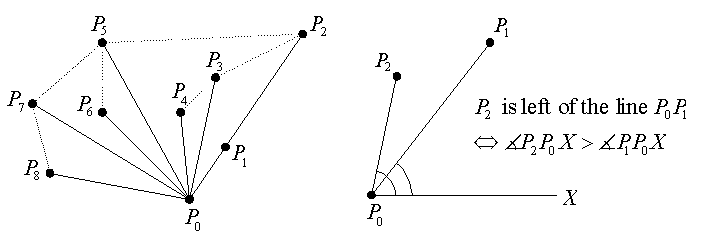
\includegraphics[width=0.9\textwidth]{content/images/methods/convexhull.png} 
  \caption{Sortierung der Punkte nach Winkel zum Startpunkt (links) mit dem Unterscheidungskriterium (rechts). Übernommen von \citet{convexHull}}
  \label{fig:convexhull}
\end{figure}

\begin{lstlisting}[mathescape,caption=Graham Scan Algorithmus, label=lst:graham-scan]
Eingabe: Menge der Punkte $P$, außen liegender Punkt $P_0$
Ausgabe: Punkte der konvexen Hülle

$i$ = 0
sortiere nach dem Winkel zu $P_0$
solange $i$ <= $|P|$
    wenn $\measuredangle P_{i-1} P_{i}$ > $\measuredangle P_{i-1} P_{i+1}$, also $P_i$ rechts von  $\vec{P_{i-1} P_{i+1}}$ liegt
        inkrementiere $i$
    ansonsten
        entferne $P_i$ aus $P$
        dekrementiere $i$
    
\end{lstlisting} 


\subsubsection{Triangulation}

Nachdem die konvexe Hülle bestimmt wurde, müssen die Punkte dieses Pfades noch trianguliert werden. Hierfür wird eine Delaunay-Triangulation mit Hilfe des Sweep-Line Algorithmus von \citet{domiter2008sweep} verwendet. Unter einer Delaunay-Triangulation versteht man zunächst einmal eine Art Prämisse, der sogenannten Umkreisbedingung, die besagt, dass ein Kreis, der alle drei Punkte eines gefundenen Polygons durchzieht, keine weiteren Punkte beinhalten darf.

\subsection{Planare Rekonstruktion als Echtzeit Umsetzung}

\subsubsection{Clusteringverfahren}

\subsection{Kantenverbesserung durch Einbeziehung von Bildmaterial}

\subsubsection{...}